%%%%%%%%%%%%%%%%%%%%%%%%%%%%%%%%%%%%%%%%%%%%%%%%%%%%%%%%%%%%%%%%%%%%%%%%%
%%%%%%%%%%%%%%%%%%%%%%%%%      INTRODUÇÃO      %%%%%%%%%%%%%%%%%%%%%%%%%%
%%%%%%%%%%%%%%%%%%%%%%%%%%%%%%%%%%%%%%%%%%%%%%%%%%%%%%%%%%%%%%%%%%%%%%%%%

\section{\esp Introdução} \label{intro}

% Instituída em 10 de dezembro de 2009, a Lei n.º 12.116/2009 \citeonline{lei}, conforme o Congresso Nacional Brasileiro, decreta o dia 27 de novembro como o Dia Nacional de Luta contra o Câncer de Mama. Além de uma data específica para a luta contra esse câncer, foi criada em 1990, uma campanha cujo objetivo é conscientizar a população sobre a importância da prevenção e do diagnóstico precoce, o chamado Outubro Rosa.

Causado pela multiplicação rápida e desordenada de células anormais, o câncer pode ocorrer em diversas estruturas do corpo, e quando envolve as células das glândulas mamárias, determina o câncer de mama \cite{incaoquee}. Esse tumor divide a primeira posição com o de pulmão no ranking dos cânceres mais incidentes do mundo, além de ser a doença mais comum entre as mulheres, na qual dados da Organização Mundial de Saúde (OMS) e do Instituto Nacional de Câncer (INCA) apontam que ocorrem por volta de 627 mil mortes por câncer de mama no mundo em 2018, sendo 17,7 mil no Brasil \cite{boletimepidemiologico}.

O diagnóstico prévio dessa doença é crucial para conter seu avanço, aumentando as chances de sobrevivência do paciente. Diante disso, são utilizados procedimentos como o exame de toque, exames clínicos e exames de imagens como a mamografia, ultrassonografia ou ressonância magnética, seguidos pela confirmação via biópsia.

% Problema Escolhido: já está incluso nesse parágrafo.
Segundo \citeonline{mamografia}, a mamografia destaca-se como o método mais eficiente para a detecção do câncer de mama em estágios iniciais. Perante o avanço computacional, a mamografia oferece uma visão detalhada de tecidos densos do corpo humano através de pequenas doses de radiação. Esse procedimento se torna essencial na detecção precoce do câncer de mama devido às características comuns da doença, como massas com margens irregulares, nódulos, micro-calcificações e assimetrias \cite{detection}.

% Motivações
Com o avanço da computação em áreas como redes neurais, processamento de imagens e Inteligência Artificial (IA), surgiram oportunidades para explorar soluções inovadoras na área da saúde, visando beneficiar tanto a comunidade médica quanto a sociedade em geral. Na oncologia, embora existam diversos métodos para diagnosticar o câncer, muitos ainda dependem de análises humanas, suscetíveis a erros e limitadas na capacidade de fazer predições ou quantificar com precisão o quadro clínico \cite{parametrization}.

Pautando-se na ideia de trazer ferramentas que auxiliam médicos no diagnóstico antecipado do câncer de mama, algoritmos de processamento de imagem e predição podem melhorar a tomada de decisões dos profissionais de saúde em relação aos pacientes. Essa abordagem permite o início antecipado do tratamento, evitando a progressão do câncer para estágios mais avançados, que são mais desafiadores de tratar. Além disso, essa intervenção aumenta as chances de cura e reduz a necessidade de tratamentos invasivos, contribuindo para uma maior qualidade de vida e longevidade para os pacientes afetados pelo câncer.

% Objetivos
Diante do contexto levantado, o presente artigo propõe uma metodologia para identificar a presença de câncer, empregando o processamento e análise de mamografias por meio de Aprendizado por Transferência (do inglês \textit{Transfer Learning}). Outrossim, a abordagem experimental incluiu o uso de uma base de imagens criteriosamente selecionada e normalizada, contendo mamografias para o treinar um algoritmo de IA. As amostras foram categorizadas em mamografias sem sinais de câncer e com câncer. Todos os códigos desenvolvidos e a base de imagens utilizadas estão disponíveis publicamente no \textit{GitHub}\footnote{\href{https://github.com/Vaftir/Breast-Cancer-Detection-AI-System}{\textit{https://github.com/Vaftir/Breast-Cancer-Detection-AI-System}}}.

Para criar um modelo de classificação binária (com câncer e sem câncer), foi utilizado o método de Aprendizado Profundo (do inglês \textit{Deep Learning}), que consiste em uma técnica avançada de Aprendizado de Máquina (do inglês \textit{Machine Learning}). Após o treinamento do modelo, a acurácia do modelo foi avaliada por meio de testes. Uma vez devidamente treinado, o algoritmo demonstrou a capacidade de analisar as imagens de mamografia, realizando uma classificação precisa e automatizada do câncer de mama.

O restante deste artigo está estruturado da seguinte maneira: a Seção \ref{fundteorica} apresenta o referencial teórico, na Seção \ref{trabcorr} é fornecida uma visão geral dos trabalhos correlatos encontrados na literatura, a Seção \ref{metodologia} descreve a metodologia, dividida em materiais e métodos, e, por fim, a Seção \ref{results} apresenta os resultados com métricas e predições. 


%%%%%%%%%%%%%%%%%%%%%%%%%%%%%%%%%%%%%%%%%%%%%%%%%%%%%%%%%%%%%%%%%%%%%%%%%
%%%%%%%%%%%%%%%%%%%      FUNDAMENTAÇÃO TEÓRICA       %%%%%%%%%%%%%%%%%%%%
%%%%%%%%%%%%%%%%%%%%%%%%%%%%%%%%%%%%%%%%%%%%%%%%%%%%%%%%%%%%%%%%%%%%%%%%%


\section{\esp Fundamentação teórica}  \label{fundteorica}

De modo a fornecer informações mais detalhadas sobre os tópicos vitais para a compreensão do presente artigo, esta seção retrata conceitos fundamentais sobre o câncer de mama, exames e tratamentos para a doença, bem como técnicas de processamento de mamografias. Além disso, será discutida a técnica de \textit{Deep Learning}, com ênfase em Redes Neurais e Redes Residuais. Além disso, são abordadas as camadas típicas de uma Rede Neural e as funções de ativação comuns.

%%%%%%%%%%%%%%%%%%%%%%      CÂNCER DE MAMA       %%%%%%%%%%%%%%%%%%%%%%%

\subsection{\esp Câncer de mama} \label{cancerdemama}
As células que compõem o corpo humano se dividem para permitir o crescimento e a substituição de células danificadas ou mortas. Esse processo é controlado pelos genes do Ácido Desoxirribonucleico (DNA, do inglês Deoxyribonucleic Acid), transmitidos pelos pais. O câncer, em geral, se forma quando esse controle genético é danificado ou perdido em uma ou mais células que então continuam a se dividir normalmente, produzindo mais células anormais, causando danos a outros tecidos e funções corporais \cite{basicOncology}.

O câncer de mama ocorre quando células anormais se multiplicam na glândula mamária. Essas células cancerígenas podem estar sob o tecido adiposo, que armazena gordura, ou nos ductos, responsáveis por conduzir o leite até a papila. Conforme \citeonline{souza}, o câncer de mama apresenta células com uma taxa de duplicação de tamanho estimada em 4 meses. Embora o crescimento seja inicialmente lento, se o tumor não for tratado e se tornar palpável, há o risco de disseminação para os linfonodos, pulmões, ossos, fígado e cérebro, resultando em metástase.

O câncer pode se manifestar de maneiras distintas, incluindo a formação de uma massa, que se refere a uma área de tecido anômalo detectada por exames de imagem devido à sua densidade ou espessura singular. Por outro lado, a calcificação ocorre quando há depósitos minerais, principalmente cálcio, nas células ou tecidos mamários.

% É importante destacar que um tumor benigno na mama não é considerado câncer, pois suas células não se espalham rapidamente para outras partes do corpo.

% A descoberta prévia do câncer de mama aumenta significativamente a probabilidade de um paciente se curar da doença, dependendo de qual método for utilizado para a detecção. Com isso, é necessário avaliar se o método escolhido é invasivo ou não. No passado, os equipamentos de medição de emissão infravermelha eram capazes de captar uma variação de temperatura apenas de 0,5 a 1 °C, utilizando uma tecnologia primitiva que exigia que um filme de cristal líquido fosse colocado nos seios dos pacientes para detectar a temperatura. Ainda assim, segundo \citeonline{noninvasive}, as câmeras de termografia infravermelhas digitais conseguem identificar mudanças de 0,08 °C, em adição de não demandar contato físico com o paciente.


%%%%%%%%%%%%%%%%%%%%%%     PROCESSAMENTO DE IMAGEM       %%%%%%%%%%%%%%%%%%%

\subsection{\esp Processamento de Imagem} \label{procesamentoimg}

Matematicamente, uma imagem pode ser descrita como uma função bidimensional, f(x, y), onde x e y representam coordenadas espaciais, e a amplitude de f em qualquer par de coordenadas é denominada intensidade ou nível de cinza da imagem naquele ponto \cite{techniques}. Quando x, y e os valores de intensidade de f são quantidades finitas e discretas, chamamos a imagem de digital. É essencial que uma imagem digital seja composta por um número finito de elementos (conhecidos como \textit{pixels}, \textit{pels} ou elementos de imagem), cada um com sua própria localização e valores específicos. 

O processamento de imagem envolve o tratamento de imagens digitais para remover ruídos e irregularidades presentes \cite{histopathological}. Ao longo das últimas décadas, várias técnicas foram desenvolvidas, inicialmente para aprimorar imagens de espaçonaves não tripuladas, sondas espaciais e aeronaves militares. Devido a fácil disponibilidade de computadores poderosos e software gráfico, os sistemas de processamentos de imagem se tornaram mais populares. As principais vantagens incluem versatilidade, repetibilidade e preservação da precisão dos dados originais, utilizando técnicas como: i) Pré-processamento, ii) Melhoria, iii) Segmentação, iv) Extração de recursos, e v) Classificação \cite{lungcancer}.

As imagens de satélites e câmeras convencionais ou digitais frequentemente apresentam limitações de contraste e brilho devido a condições de iluminação ou subsistemas de imagem, além de conterem diversos tipos de ruído \cite{techniques}. Nesse contexto, o aprimoramento de imagem busca realçar características específicas da imagem para análise posterior ou exibição. As técnicas de aperfeiçoamento, que englobam alargamento de contraste, conforme mostrado na Figura \ref{fig:contraste}, modificação do histograma e filtragem de ruído, consoante à Figura \ref{fig:ruido}, são úteis na extração de recursos, análise e exibição. Entretanto, o próprio processo de aprimoramento não aumenta o conteúdo de informações inerentes aos dados, enfatizando somente certas características de imagem especificadas.

\begin{figure}[ht]
\centering
\begin{minipage}[b]{0.45\linewidth}
\centering
\caption{Alargamento de Contraste}
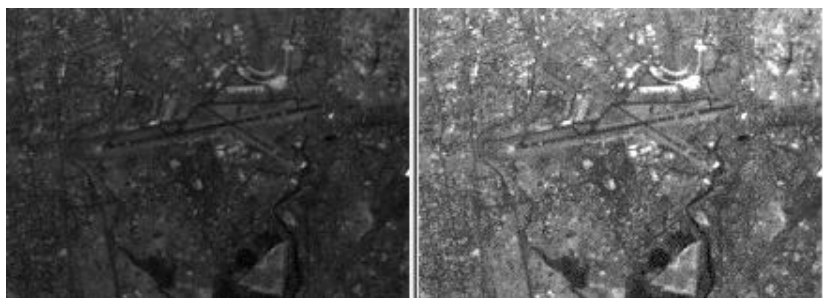
\includegraphics[width=\textwidth]{figuras/Alargamento de Contraste.png}
\label{fig:contraste}
\vspace{-0.2cm}
\textbf{\footnotesize Fonte: \cite{techniques}}
\end{minipage}
\hspace{0.5cm}
\begin{minipage}[b]{0.45\linewidth}
\centering
\caption{Retirada de Ruído}
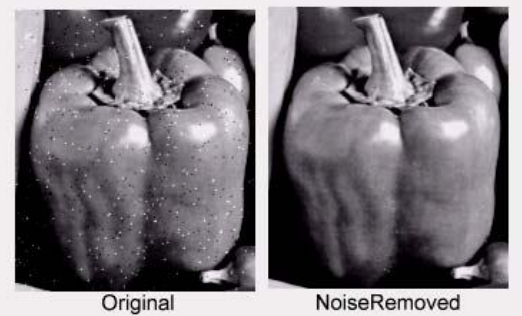
\includegraphics[width=\textwidth]{figuras/Retirada de Ruido.png}
\label{fig:ruido}
\vspace{-0.2cm}
\textbf{\footnotesize Fonte: \cite{techniques}}
\end{minipage}
\end{figure}



%%%%%%%%%%%%%%%%%%%%%%%%%%     DEEP LEARNING       %%%%%%%%%%%%%%%%%%%%%%

\subsection{\esp \textit{Deep Learning}} \label{deeplearning}


O termo \textit{Deep Learning} refere-se à uma estrutura utilizada para realização do processo de \textit{Machine Learning}, método que usa dados para criar uma IA que aprende e executa funções de maneira automática. Compondo-se de várias camadas de neurônios artificiais conectados, o \textit{Deep Learning} permite que o sistema aprenda representações cada vez mais complexas dos dados de entrada. Esses dados podem variar desde um simples conjunto de inteiros, para uma predição de cálculo, até um sistema de navegação de um veículo autônomo \cite{deeplearning}.

Os neurônios artificiais são a principal composição da rede neural, sendo estruturas agrupadas em camadas, inspiradas nos neurônios biológicos presentes no cérebro humano. Cada neurônio artificial recebe diversas entradas, representadas por valores numéricos, multiplicadas por um determinado peso e somados. Esse resultado é então processado mediante uma função de ativação, que determina a saída do neurônio, e é transmitida para os outros neurônios da rede.



%%%%%%%%%%%%%%%%%%%%%%%%%%     REDES NEURAIS       %%%%%%%%%%%%%%%%%%%%%%


\subsection{\esp Redes Convolucionais e Redes Residuais} \label{redesconvoleredesresidual}

A Rede Neural Convolucional (CNN, do inglês \textit{Convolutional Neural Network}) é uma estrutura complexa que utiliza neurônios e camadas de convolução para detectar características visuais em imagens por meio de conjunto de filtros \cite{cnn}. Sua arquitetura é composta por três camadas: i) Camada de Entrada (do inglês \textit{Input Layer}), ii) Camadas Escondidas (do inglês \textit{Hidden Layers}), e iii) Camada de Saída (do inglês \textit{Output Layer}).

Na camada de entrada, os dados brutos, como fotos e vídeos, são recebidos e transformados em dados matemáticos enviados para as camadas seguintes da CNN. Nas camadas escondidas, são usadas funções matemáticas não-lineares modeladas para retornar valores específicos, consoantes os dados de entrada. Esses valores são então enviados para a última parte da rede. Por fim, na camada de saída, é produzido o resultado com base nas predições das camadas anteriores \cite{medical}.

A Rede Neural Residual (ResNet, do inglês \textit{Residual Network}) é uma variação da CNN que resolve problemas associados à degradação de desempenho e melhora a eficiência no treinamento. Utilizando atalhos, a ResNet navega através de múltiplas camadas da rede, facilitando o aprendizado incremental das características. A arquitetura inclui blocos residuais enriquecem o fluxo de dados, permitindo a passagem direta de informações às camadas subsequentes.

Dentro de cada bloco residual, várias camadas são empilhadas e o fluxo de dados é enriquecido pelos atalhos que permitem a passagem direta das informações às camadas subsequentes. Esses blocos variam em tipos e camadas, adaptando-se à profundidade e complexidade específicas da arquitetura. A Figura \ref{fig:cnn} ilustra as camadas de uma \textit{ResNet}, aplicado no problema de identificação de câncer de mama.

\begin{figure}[ht]
 	\centering	
 	\caption[\hspace{0.1cm}Grade Computacional.]{Arquitetura completa de uma CNN que classifica dígitos manuscritos}
 	\vspace{-0.2cm}
 	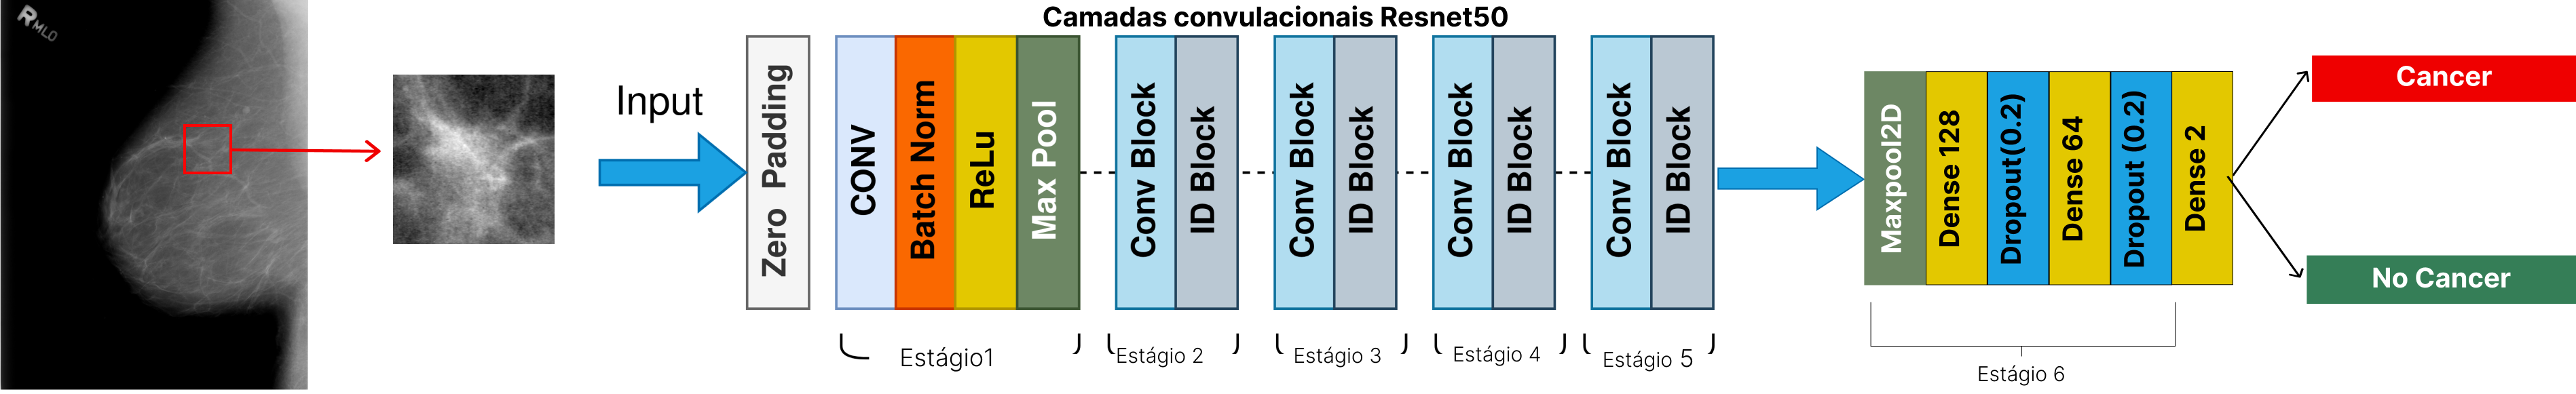
\includegraphics[width=1\textwidth]{figuras/cnn.png}
 	\captionsetup{justification=centering}
	\vspace{-0.2cm}
     \\\textbf{\footnotesize Fonte: Elaborado pelos autores}
	\label{fig:cnn}
\end{figure}

\subsection{\esp Camadas da CNN e Funções de Ativação} \label{camadasfund}

Uma arquitetura \textit{ResNet} é formada por diversos blocos residuais, cada um composto por múltiplas camadas. A configuração dos blocos e camadas pode variar de acordo com a profundidade e complexidade da arquitetura em questão. Cada bloco residual inicia com camadas convolucionais que aplicam filtros a uma imagem de entrada para extrair características importantes. A profundidade da saída de uma convolução corresponde ao número de filtros aplicados, resultando em detalhes mais refinados no Mapa de Ativação (do inglês \textit{Atactivation Map}).

Os filtros, também conhecidos como \textit{Kernels}, possuem em pesos ajustados durante a Retropropagação do Erro (do inglês \textit{Backpropagation}), sendo aplicados a pequenas regiões de entrada denominados Campos Receptivos (do inglês \textit{Receptive Field}). Na Figura \ref{fig:conv2} é possível observar um filtro que representa a curva ao seu lado. Essa combinação resulta em um valor alto, indicando compatibilidade entre as curvas. Quando não há compatibilidade na imagem, esse resultado se aproxima de zero.

\begin{figure}[ht]
 	\centering	
 	\caption[\hspace{0.1cm}Grade Computacional.]{Camada Convolucional}
 	\vspace{-0.4cm}
 	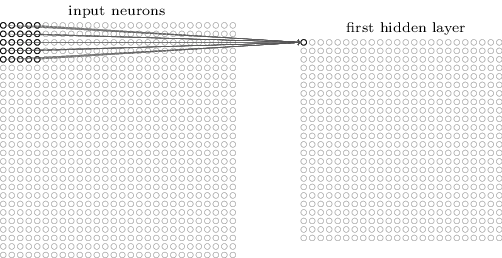
\includegraphics[width=0.9\textwidth]{figuras/conv.png}
 	\captionsetup{justification=centering}
	\vspace{-0.2cm}
     \\\textbf{\footnotesize Fonte: \cite{cnns}}
	\label{fig:conv2}
\end{figure}


Após as operações de convolução, são aplicadas funções de ativação, como a \textit{Softmax}, representada na Figura \ref{fig:softmax}, que converte a saída em uma probabilidade de pertencimento a uma das classes predefinidas. Sem essa função, as saídas dos neurônios são valores numéricos, onde o maior indica a classe vencedora. Em contrapartida, a função de ativação Unidade Linear Retificada (ReLU, do inglês \textit{Rectified Linear Unit}), representada na Figura \ref{fig:relu}, atribui o valor zero a todas as entradas menores ou iguais à zero. É amplamente utilizada devido à sua rapidez na geração de pesos e é especialmente adequada para problemas com apenas duas classes.

\begin{figure}[ht]
\centering
\begin{minipage}{0.45\textwidth}
  \centering
  \caption[\hspace{0.1cm}Grade Computacional.]{Função de Ativação \textit{softmax}}
  \vspace{-0.4cm}
  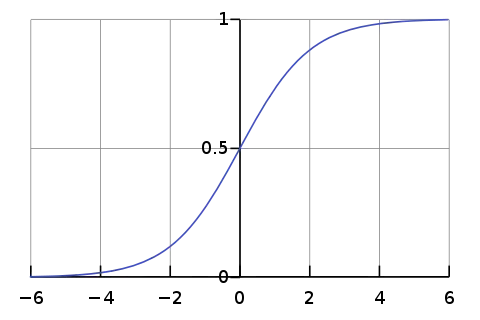
\includegraphics[width=\linewidth]{figuras/softmax.png}
  \captionsetup{justification=centering}
  \vspace{-0.2cm}
  \\\textbf{\footnotesize Fonte: \cite{softmax}}
  \label{fig:softmax}
\end{minipage}\hfill
\begin{minipage}{0.45\textwidth}
  \centering
  \caption[\hspace{0.1cm}Grade Computacional.]{Função de Ativação \textit{ReLU}}
  \vspace{-0.4cm}
  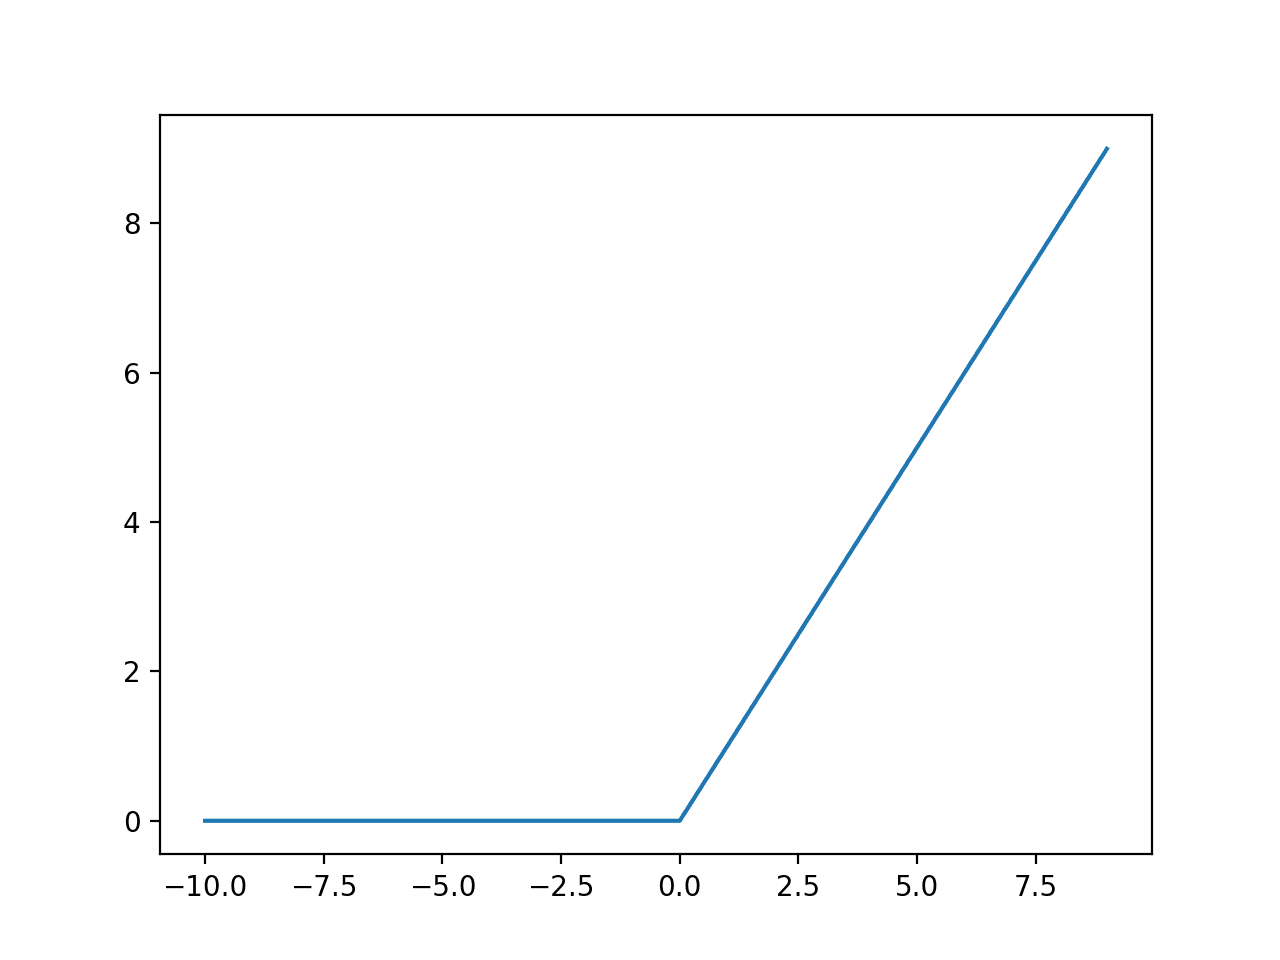
\includegraphics[width=\linewidth]{figuras/relu.png}
  \captionsetup{justification=centering}
  \vspace{-0.2cm}
  \\\textbf{\footnotesize Fonte: \cite{relu}}
  \label{fig:relu}
\end{minipage}
\end{figure}


A camada de \textit{Max Pooling} desempenha um papel importante na redução da dimensionalidade dos dados de entrada. Ela opera agrupando \textit{pixels} em regiões, o que ajuda a reduzir a sensibilidade a pequenas variações nos dados, ao mesmo tempo em que extrai características mais relevantes. Essa camada diminui a resolução da imagem, permitindo uma ênfase maior em características específicas, enquanto compacta o conjunto de dados mantendo as informações mais relevantes em uma seleção das regiões de maior destaque.


Após os blocos residuais, a \textit{ResNet} possibilita a integração de camadas Totalmente Conectadas (do inglês, \textit{Fully-Connected}), também conhecidas como camadas \textit{Dense}. Essas camadas são responsáveis por tomar as características extraídas por camadas anteriores e transformá-las em uma saída final. No entanto, essas camadas não fazem parte dos próprios blocos residuais da \textit{ResNet}, uma vez que a arquitetura é focada em melhorar a eficácia das camadas convolucionais.

%%%%%%%%%%%%%%%%%%%%%%%%%%%%%%%%%%%%%%%%%%%%%%%%%%%%%%%%%%%%%%%%%%%%%%%%%
%%%%%%%%%%%%%%%%%%%%      TRABALHOS CORRELATOS       %%%%%%%%%%%%%%%%%%%%
%%%%%%%%%%%%%%%%%%%%%%%%%%%%%%%%%%%%%%%%%%%%%%%%%%%%%%%%%%%%%%%%%%%%%%%%%


\section{\esp Trabalhos correlatos} \label{trabcorr}

Nesta seção, são abordados trabalhos correlatos que utilizam IA para o diagnóstico de câncer, se diferenciando em termos de entrada de imagem (como radiografias ou imagens digitais), além de apresentar as bases de dados usadas, abordagens, algoritmos e análises dos resultados. 

Em \citeonline{marinePredators}, foi proposto um modelo de detecção de câncer de mama. O trabalho alcançou uma acurácia de 92\%, normalizando imagens termográficas e utilizando o \textit{Marine-Predators-Algorithm} que auxilia na otimização da seleção das características (definidas por algumas técnicas de reconhecimento de padrões) mais relevantes das imagens e parâmetros do modelo de observação. Para classificar e validar a implementação feita, foram utilizadas variantes (tipos de funções matemáticas que medem a similaridade entre dois pontos no espaço) do algoritmo de Máquina de Vetores de Suporte (SVM, do inglês \textit{Support Vector Machine}).

Por outro lado, \citeonline{comparing}, ao utilizar outra abordagem de treinamento do algoritmo, alcançaram 61,8\% de precisão dos resultados. Foi utilizado o método de limiarização por refinamento adaptativo, técnica que segmenta uma imagem em duas ou mais (com base nos valores dos \textit{pixels}), de modo que regiões anormais são identificadas com mais precisão. Outrossim, o artigo compara o resultado entre suas métricas com outros trabalhos, e com base nisso, concluiu-se que a inconsistência das comparações foi devido ao uso de imagens infravermelhas distintas, uma vez que foram utilizadas 102 imagens de uma base de dados pública.
%Diz q usa limiarização baseado na Section III .ASPECTS OF THE APPLIED APPROACH: "In our approach we have used the same methodology that composed the automatic ROI segmentation developed in [19] that was proven to produce good results regarding a comparison to a (...)"

Assim como o trabalho anterior, \citeonline{segmentacao} utilizaram da limiarização por refinamento adaptativo, todavia, com uma acurácia de 96\%. Foram introduzidos três parâmetros para avaliação, baseando-se na informação de que as pregas mamárias (área indicadora de limites inferiores da mama, pois possuem maior temperatura) podem variar de tamanho, dificultando a identificação das mamas. Os parâmetros determinam miliares mínimos de uma área medida em \textit{pixels} que a prega deve ter, além de definir a área mínima a ser medida em \textit{pixel} para duas componentes distintas. Com isso, foi possível determinar qual conjunto de parâmetros maximiza as métricas estatísticas apresentadas, indicando assim os resultados normalizados.

Em \citeonline{MachineVision}, foram desenvolvidas técnicas de Visão de Máquina (do inglês \textit{Machine Vision}), um algoritmo que processa imagens e reconhece características básicas, em contraste com técnicas de processamento de imagens, que geram outra imagem tratada. Com o uso de linguagens de alto nível, inúmeros algoritmos foram otimizados resultando em poderosas ferramentas acessíveis a pesquisadores e cientistas, aumentando a precisão dos resultados. A discussão da Visão de Máquina e algoritmos de processamento de imagem foi dividida em cinco grupos: Técnicas de Segmentação ou Limiar em \textit{Grey-Level}; Técnicas de Detecção de Borda; Morfologia Digital; Textura; e Algoritmos de Esqueletização e Encurtamentos.


Ao utilizar redes neurais para reconhecer imagens de câncer de pele e unindo técnicas de processamento de imagens digitais, \citeonline{botelho} desenvolveram um sistema que diferencia imagens de melanomas. O método proposto utiliza quatro características para identificar lesões: assimetria, bordas irregulares, cor variada e diâmetro. Implementando a rede neural \textit{Perceptron} de Camada Única com dois neurônios, um excitado por imagens de lesões Melanoma, e outro excitado por imagens de lesões não Melanoma, o \textit{Perceptron} ajusta os pesos por meio da Regra Delta ao identificar entradas classificada erroneamente. A rede foi treinada até que todas as saídas corresponder às saídas esperada, alcançando uma taxa de acertos de 69\%.

\citeonline{NakagamiImages} apresentam uma abordagem de \textit{Deep Learning} para detecção e classificação de massas na mama, combinando imagens de ultrassom \textit{B-mode} e Nakagami, para fornecer informações complementares sobre o padrão de dispersão de tecidos. O ultrassom B-mode utiliza ondas sonoras de alta frequência para criar imagens em escala cinza, destacando áreas mais brilhantes como tecidos mais densos. As imagens Nakagami, por sua vez, analisam as amplitudes de sinal para fornecer informações sobre a presença de diferentes estruturas. Com uma arquitetura de rede neural convolucional para extrair características das imagens combinadas, o modelo classificou massas como malignas ou benignas. A abordagem mostrou-se altamente eficaz na localização de massas, com uma precisão de 91,8\%, superando significativamente abordagens que utilizam apenas imagens B-mode ou Nakagami.

Em \citeonline{systematic}, os autores analisaram diversos tipos de Redes Neurais Artificiais (ANN, do inglês \textit{Artificial Neural Network}) usados na literatura para processar imagens termográficas de câncer de mama. Apesar da termografia ser o método mais eficaz para a detecção precoce, a qualidade das imagens é um desafio tangível. O aprimoramento de imagem busca revelar detalhes ocultos e destacar características que permitam distinguir a profundidade e o tamanho do tumor de um tecido saudável. Para melhorar a qualidade, o estudo utiliza um dispositivo de resfriamento da mama. As contribuições e desvantagens de trabalhos relacionados que empregam termografia e IA são destacadas, com comparações ao longo do artigo, levantando questionamentos a cerca dos desafios enfrentados, como a falta de padronização na aquisição de imagens térmicas e a necessidade de mais dados de treinamento para as redes neurais. 

Para desenvolver uma técnica precisa e eficiente para a identificação antecipada do câncer de mama, \citeonline{ChaoticSalp} usaram a segmentação de imagens térmicas em conjunto com o algoritmo \textit{Chaotic Salp Swarm}. O algoritmo proposto consiste em uma técnica de otimização bioinspirada, usada para ajustar os parâmetros de segmentação das termografias e encontrar as regiões suspeitas de câncer de mama. Assim como o anterior, foi utilizada uma base de dados pública de imagens térmicas para avaliar a eficácia do método proposto. Os resultados obtidos foram avaliados baseados em métricas como: sensibilidade, especificidade e coeficiente de Dice. Não foi especificado o índice de precisão do trabalho, entretanto, foi considerado que o método proposto teve um desempenho satisfatório em termos de precisão na segmentação de regiões suspeitas de câncer de mama nas imagens térmicas.

Em \citeonline{borchartt}, a ênfase foi na análise das contribuições potenciais das imagens infravermelhas para diagnósticos de doenças na mama. O estudo utilizou imagens da base de dados público da Pro Engenharia (PROENG), das quais 47\% apresentavam alguma anormalidade. Algoritmos como Máquina de Vetores de Suporte (SVM, do inglês \textit{Support Vectors Machine}) foram empregados para identificação de condições malignas, utilizando características como primeiro e terceiro momento, não uniformidade da massa cinzenta e porcentagem de execução. Foram destacados desafios na segmentação da região de mama e extração da região de interesse devido à natureza amorfa e à falta de limites claros. Além disso, foi apontado que ao usar uma base de dados público para comparações e extração de características, o classificador \textit{Sequential Minimum Optimization} (SMO) obteve os melhores resultados,  ressaltando a inconsistência da comparação entre trabalhos que utilizam imagens infravermelhas. 

Buscando explorar métodos não invasivos para a localização precoce do câncer de mama, \citeonline{leles} propuseram o uso de imagens térmicas que permitem detectar mudanças na temperatura, causadas pelo aumento do fluxo sanguíneo na área afetada pelo tumor. Após o pré-processamento, foi feito o refinamento manual da região de interesse para que alguns atributos extraídos não colaborassem com dados de fora da mama. Avaliando 70 pacientes, o trabalho identificou a temperatura máxima, mínima e média das mamas para utilizar no cálculo da sensibilidade (capacidade do teste em identificar corretamente o diagnóstico) e especificidade (capacidade do teste em excluir corretamente os que não tem a doença), com os valores de 92,3\% e 86,2\%, respectivamente.

A fim de abordar a detecção de metástase em linfonodos axilares em pacientes com câncer de mama, \citeonline{ashokkumar} utilizaram o método de \textit{Data Augmentation} que faz modificações geométricas das imagens (como rotação, inversão, deslocamento e dimensionamento). Isso fornece uma garantia de que o modelo se concentra em áreas de câncer de mama, em vez de fontes de ruído aleatórias. Conforme o texto, foi demonstrado que o método ajuda na memorização de qualidades específicas das imagens treinadas, e evita que as redes se tornem superajustadas, ou seja, um modelo de Aprendizado Profundo que se adaptou demasiadamente nos dados de treinamento a ponto de não conseguir capturar padrões mais amplos. Além disso, usando ANN, o trabalho alcançou 98\% de acurácia superando modelos de radiografia.


%%%%%%%%%%%%%%%%%%%%%%%%%%%%%%%%%%%%%%%%%%%%%%%%%%%%%%%%%%%%%%%%%%%%%%%%%
%%%%%%%%%%%%%%%%%%%%%%%%      METODOLOGIA       %%%%%%%%%%%%%%%%%%%%%%%%%
%%%%%%%%%%%%%%%%%%%%%%%%%%%%%%%%%%%%%%%%%%%%%%%%%%%%%%%%%%%%%%%%%%%%%%%%%


\section{\esp Metodologia} \label{metodologia}
A fim de aprofundar os fundamentos do tema abordado, esta seção apresenta os recursos e ferramentas utilizados para a implementação do algoritmo, bem como informações técnicas relacionadas a linguagens de programação, bibliotecas e base de dados.


%%%%%%%%%%%%%%%%%%%%%%%     MATERIAIS       %%%%%%%%%%%%%%%%%%%%%%

\subsection{\esp Materiais} \label{materiais}

As imagens mamográficas utilizadas foram obtidas do desenvolvimento mencionado em \citeonline{newdatabase}, que visa abordar desafios comuns associado a bancos de imagens de mamografia, tanto de origem privada quanto pública. Esses bancos frequentemente sofrem de limitações de tamanho e restrições de acessibilidade, resultando em informações insuficientes. O Subconjunto de Imagens de Mama com Curadoria DDSM\footnote{\href{https://www.kaggle.com/datasets/awsaf49/cbis-ddsm-breast-cancer-image-dataset}{\textit{www.kaggle.com/datasets/awsaf49/cbis-ddsm-breast-cancer-image-dataset}. Acesso em 13 de setembro de 2023.}} (do inglês, \textit{Curated Breast Imaging Subset DDSM}), de 2016, consiste em um total de 277524 imagens, categorizadas em massa e calcificação, subdivididas em três subcategorias cada. Mamografias Completas (do inglês \textit{Full Mammogram}) apresentam imagens sem recortes, seguidas por Imagens Cortadas (do inglês \textit{Cropped Images}) que destacam áreas específicas do tumor, e Regiões de Interesse (ROI, do inglês \textit{Region of Interest}), concentrando-se exclusivamente em áreas com massas ou calcificações.

O modelo projetado opera exclusivamente com imagens de massas e imagens cortadas. Dentro desses critérios, foi desenvolvido um algoritmo para realizar a segmentação das imagens utilizadas, uma vez que o banco de imagens apresenta uma abordagem não convencional em relação à sua categorização. Ao contrário de uma separação clara entre tumores benignos e malignos, as imagens são organizadas em múltiplas pastas, sendo identificadas por meio de arquivos CSVs que contêm o identificador do paciente, a patologia do tumor e o caminho das imagens. A implementação do algoritmo está disponível publicamente no \textit{GitHub}\footnote{\href{https://github.com/g1ovannab/database-segmentation}{\textit{github.com/g1ovannab/database-segmentation}}}.

Após a conclusão da segmentação, o conjunto de dados resultante apresentou 1555 imagens, distribuídas entre 784 imagens de pacientes com tumor maligno (câncer) e 771 imagens de pacientes com tumor benigno (ausência de câncer). Para ilustrar, a Figura \ref{fig:pcc} demonstra um exemplo de uma imagem utilizada para a predição de um paciente com câncer, enquanto a Figura \ref{fig:psc} exibe uma imagem de um paciente sem câncer. 

% \footnote{\href{https://www.kaggle.com/datasets/awsaf49/cbis-ddsm-breast-cancer-image-dataset}{\textit{https://www.kaggle.com/datasets/awsaf49/cbis-ddsm-breast-cancer-image-dataset}. Acesso em 13 de setembro de 2023.}}

\begin{figure}[ht]
\centering
    \begin{minipage}[b]{0.45\textwidth}
        \centering
        \caption{Paciente com câncer}
        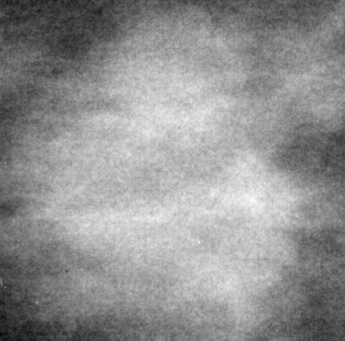
\includegraphics[width=0.5\textwidth]{figuras/with_cancer.jpg}
        \label{fig:pcc}
        
        \textbf{\footnotesize Fonte: \href{https://www.kaggle.com/datasets/awsaf49/cbis-ddsm-breast-cancer-image-dataset}{\cite{newdatabase}}}
    \end{minipage}
    \hfill
    \begin{minipage}[b]{0.45\textwidth}
        \centering
        \caption{Paciente sem câncer}
        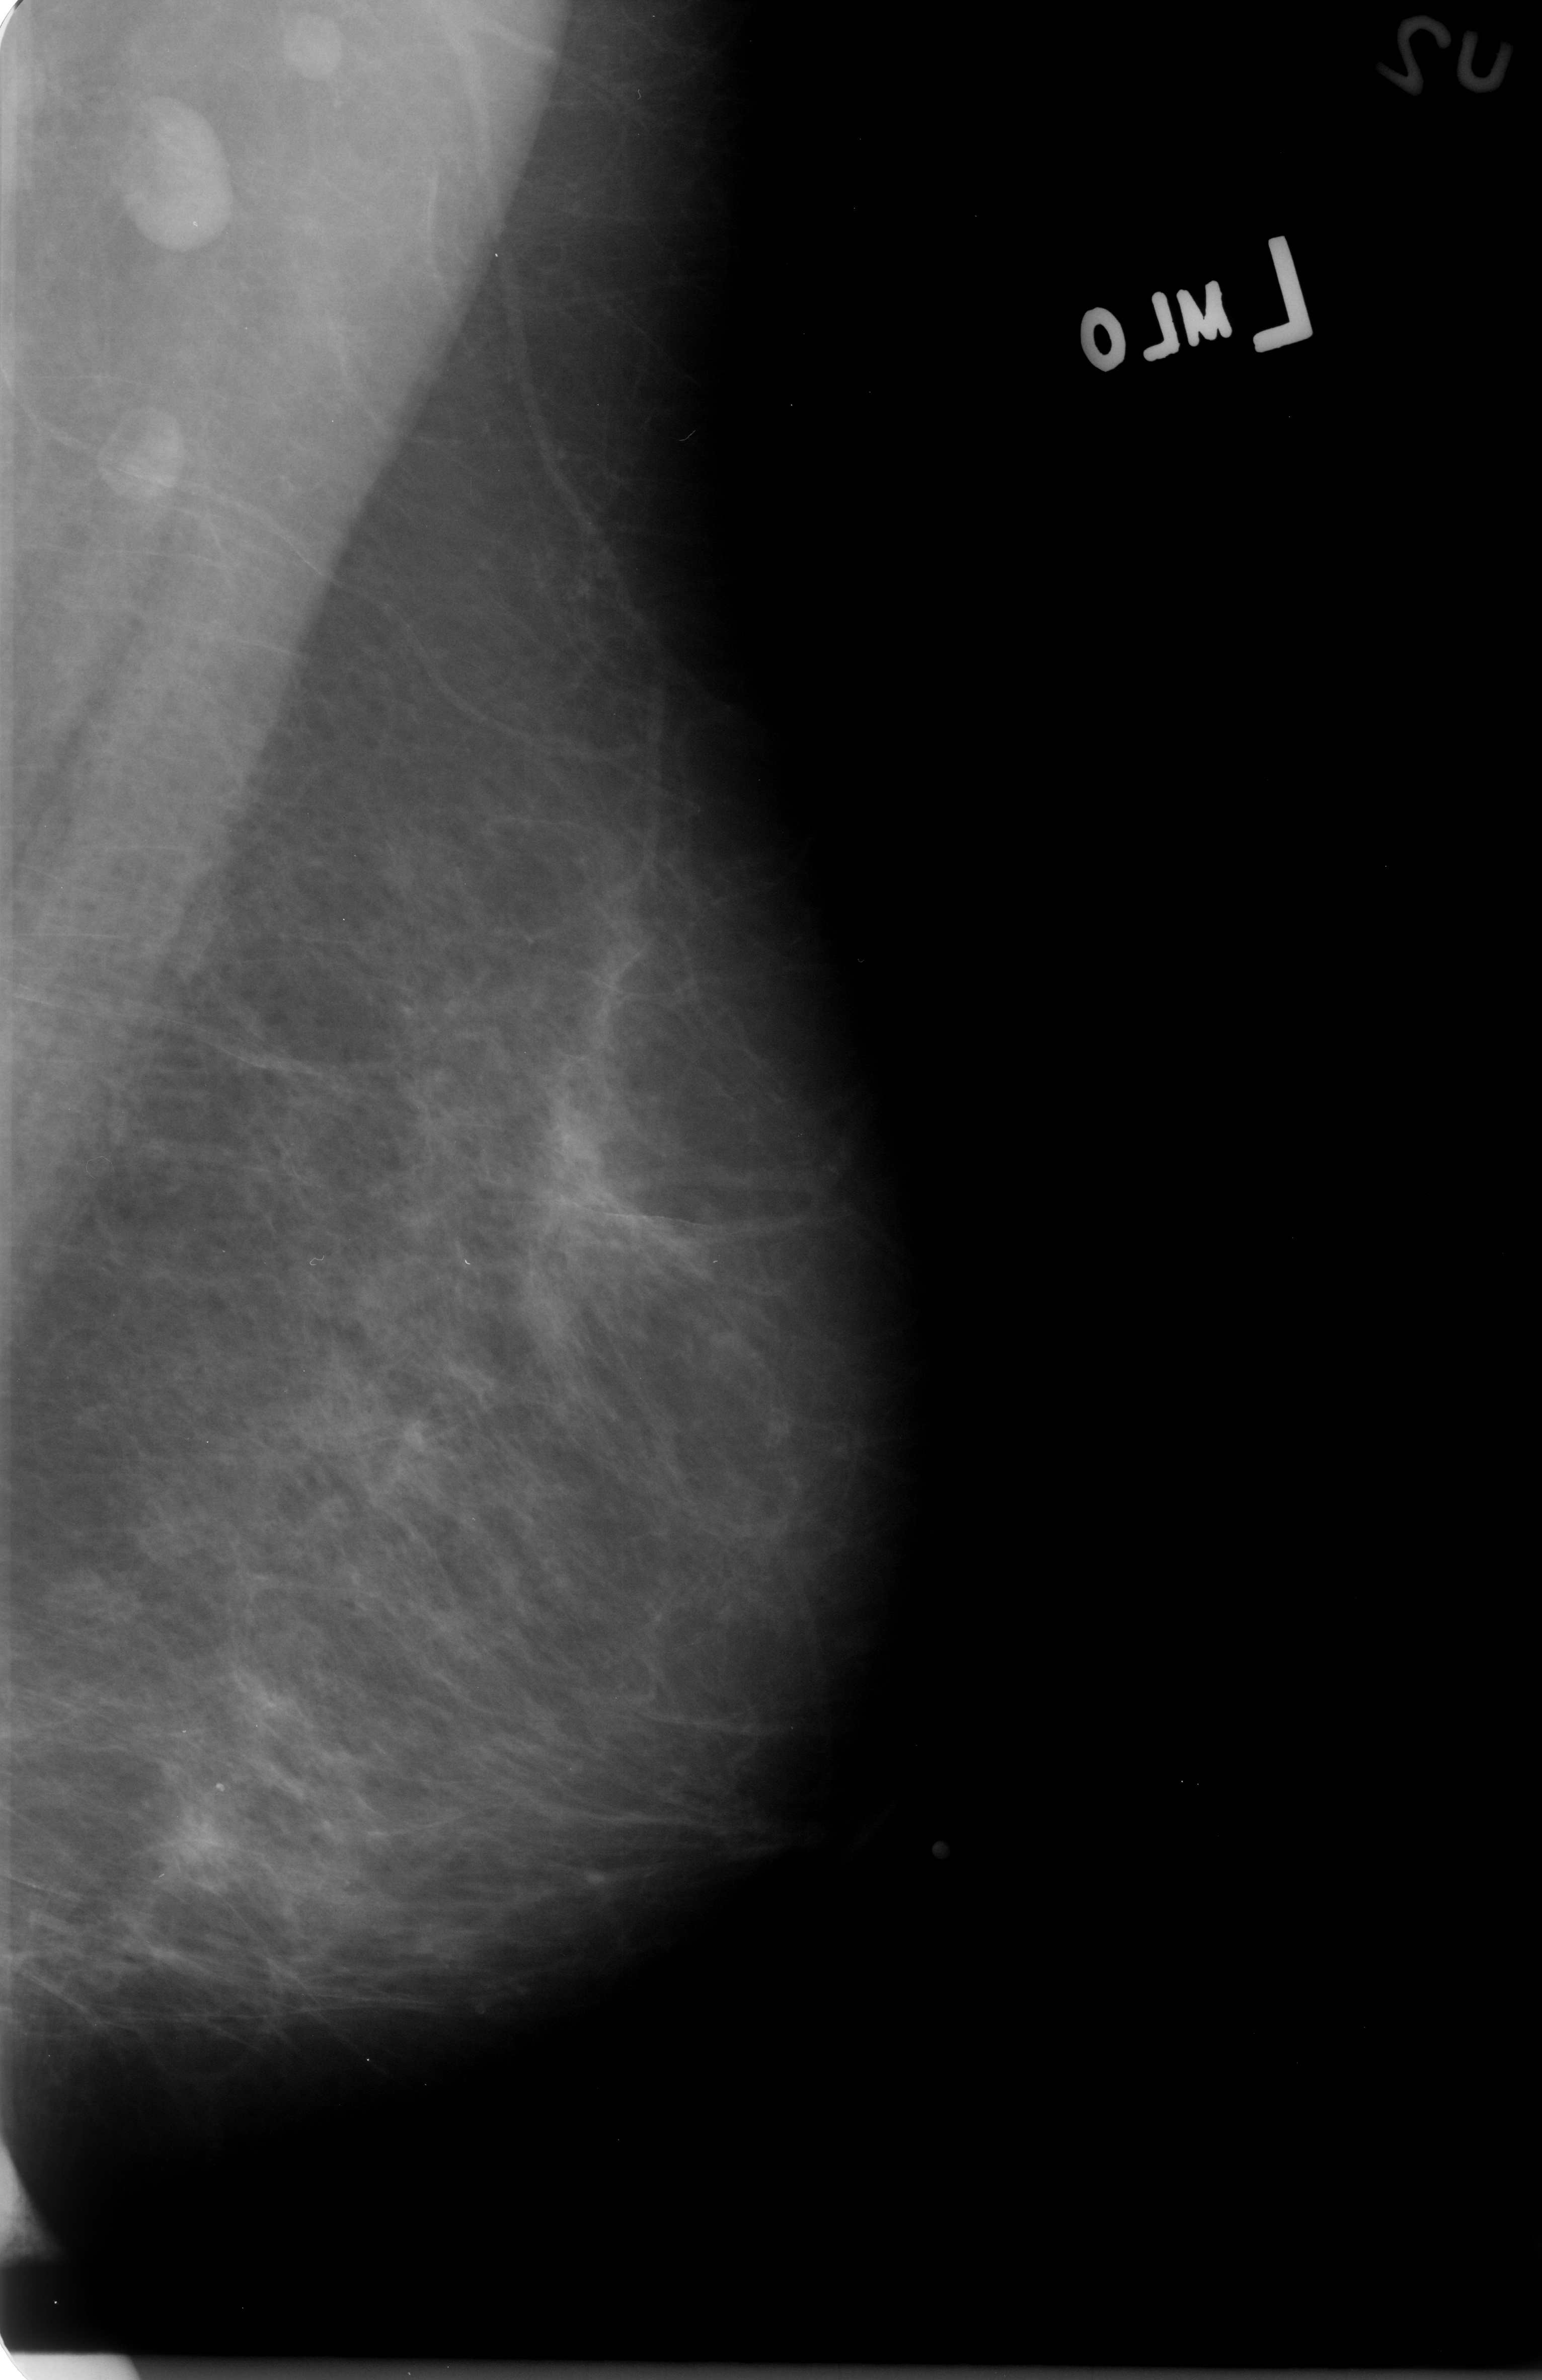
\includegraphics[width=0.5\textwidth]{figuras/without_cancer.jpg}
        \label{fig:psc}
        
        \textbf{\footnotesize Fonte: \href{https://www.kaggle.com/datasets/awsaf49/cbis-ddsm-breast-cancer-image-dataset}{\cite{newdatabase}}}
    \end{minipage}
\end{figure}


O algoritmo de classificação das imagens entre pacientes com e sem câncer foi desenvolvido utilizando diversas tecnologias e bibliotecas, em conjunto com o \textit{Python} 3.10, uma linguagem de programação de alto nível, interpretada e com tipagem dinâmica, além de incluir orientação a objetos e suporte a módulos e pacotes.

No desenvolvimento do modelo, destacam-se bibliotecas essenciais como o \textit{TensorFlow} para construção de modelos de \textit{Machine Learning}, frequentemente associado ao \textit{Keras} para o treinamento de redes neurais. A \textit{matplotlib} é empregada para a visualização de dados, permitindo a criação de gráficos, \textit{plots} e histogramas. O \textit{numpy} desempenha um papel crucial na computação numérica, oferecendo uma estrutura de dados versátil para armazenar grandes conjuntos de dados numéricos. A biblioteca \textit{cv2} fornece funções para carregar, manipular e processar imagens, enquanto o \textit{ImageDataGenerator} simplifica a transformação de imagens em dados vetoriais, otimizando os cálculos durante o treinamento do modelo.

Apresentada na Subseção \ref{redesconvoleredesresidual}, a arquitetura \textit{ResNet} destaca-se por sua ênfase no reconhecimento de imagens, além de ter conquistado o primeiro lugar no Desafio de Reconhecimento Visual em Larga Escala ImageNet (ILSVRC, do inglês \textit{ImageNet Large Scale Visual Recognition Challenge}) em 2015 \cite{resnet50analisys}. Neste desafio, obteve uma taxa de erro top 5 de 3,6\% ao empregar uma CNN composta por 152 camadas, denominada \textit{ResNet152}.

Embora a \textit{ResNet152} seja reconhecida como o modelo mais profundo para capturar recursos abstratos e complexos, essa profundidade implica em custos computacionais significativos. A família \textit{ResNet} apresenta variantes como \textit{ResNet18}, \textit{ResNet34}, \textit{ResNet50} e \textit{ResNet101}, que compartilham o mesmo conceito mas diferem na quantidade de camadas. Conforme \citeonline{resnet50analisys}, as \textit{ResNet} com 50, 101 e 152 camadas demonstram maior precisão em comparação às versões com 18 e 34 camadas. Entre elas, a \textit{ResNet50} destaca-se pelo equilíbrio na profundidade das camadas, uma vez que as arquiteturas com 101 e 152 camadas demandam recursos computacionais substancialmente superiores.



%%%%%%%%%%%%%%%%%%%%%%%     MÉTODOS       %%%%%%%%%%%%%%%%%%%%%%


\subsection{\esp Métodos} \label{metodos}

Nesta subseção, são apresentadas as metodologias para o treinamento de um modelo de rede neural convolucional fazendo uso de bibliotecas do \textit{Python}. Disponíveis na Figura \ref{fig:diagrama}, o método proposto consiste em cinco etapas: pré-processamento, aplicação do método de \textit{Transfer Learning}, declaração do modelo da rede neural, treinamento do modelo e predições.

\begin{figure}[ht]
 	\centering	
 	\caption[\hspace{0.1cm}Grade Computacional.]{Etapas metodológicas}
 	\vspace{-0.2cm}
 	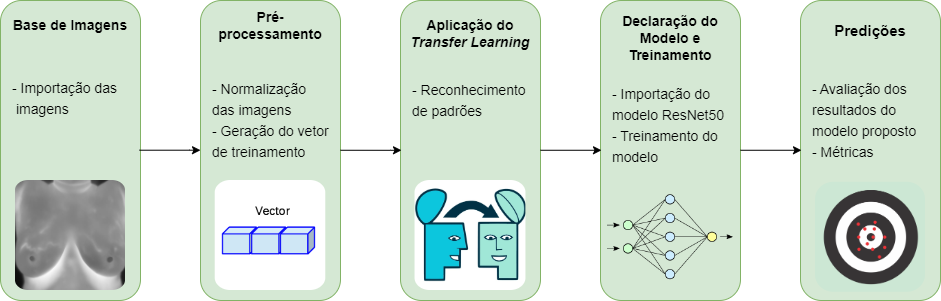
\includegraphics[width=1\textwidth]{figuras/tcc_diagrama.drawio.png}
    \captionsetup{justification=centering}
  \vspace{-0.2cm}
     \\\textbf{\footnotesize Fonte: Elaborado pelos autores}
	\label{fig:diagrama}
\end{figure}



%%%%%%%%%%%%%%%%%%%%%%%     PRÉ-PROCESSAMENTO       %%%%%%%%%%%%%%%%%%%%%%

\subsubsection{\esp Pré-Processamento} \label{preprocess}

Inicialmente, foi feita uma segunda segmentação, desta vez manual, para distribuir as imagens em conjuntos distintos. O conjunto de treinamento consistiu em 945 imagens (sendo 468 para pacientes sem câncer e 477 para paciente com câncer), 464 imagens como dados de validação (sendo 230 para pacientes sem câncer e 234 para pacientes com câncer), e 146 imagens para dados de teste (sendo 73 para pacientes sem câncer e 73 para pacientes com câncer). Totalizando 1555 imagens, a distribuição resultou em 60,8\% para treinamento, 29,8\% validação e 9,4\% para teste.

Em seguida, as imagens foram pré-processadas utilizando métodos transformam os valores originais dos \textit{pixels} em uma escala específica. Geralmente, essa escala é utilizada com o valor de 1/255, uma vez que as imagens utilizadas na implementação consistem em coeficientes Vermelho, Verde, Azul (RGB, do inglês \textit{Red, Green, Blue}), ou seja, cada \textit{pixel} tem um valor entre 0 e 255. Entretanto, esses valores são grandes demais para o modelo proposto processar, conforme a taxa de aprendizado comum. Por conta disso, os valores foram realinhados para se distinguir entre 0 e 1.

Foi utilizado um método originado da biblioteca \textit{Keras} que cria uma estrutura que gera Lotes (do inglês \textit{Batches}) de dados sob demanda à medida que o modelo é treinado. Em vez de carregar todos os dados de treinamento de uma vez, o gerador carrega apenas um pequeno lote de dados por vez. O método também redimensiona das imagens para 224x224 \textit{pixels}, uma vez que a \textit{ResNet} requer esses valores \cite{kerasresnet50}, além de definir o modo de classificação em binário (pacientes sem câncer ou pacientes com câncer).


%%%%%%%%%%%%%%%%%%%%%%%     TRANSFER LEARNING       %%%%%%%%%%%%%%%%%%%%%%

\subsubsection{\esp Aplicação do \textit{Transfer Learning}} \label{transfer}

A fim de empregar um modelo pré-treinado em uma determinada tarefa como ponto de partida para resolver um problema relacionado, o \textit{Transfer Learning} foi aplicado. Isso permite aproveitar o conhecimento adquirido por um modelo já pré-treinado, a fim de reconhecer padrões e características úteis nos dados. O método de aplicação consiste em obter camadas de um modelo já treinado, congelar essas camadas já treinadas (para evitar destruir quaisquer informações que elas possuem durante o treinamento), adicionar novas camadas treinadas em cima das camadas congeladas (retornando características anteriores em predições para um novo \textit{dataset}) e, por fim, treinar as novas camadas \cite{kerastransfer}.

Na implementação do modelo de classificação de câncer, foi utilizada a arquitetura \textit{ResNet50} para realizar o processo de \textit{Transfer Leaning}, modelo de rede neural que utiliza blocos residuais, permitindo que a informação seja passada diretamente para camadas posteriores. Com essa informação, foi carregado o pré-processamento da \textit{ResNet} para que as imagens possam ser entendíveis para a rede utilizada. Em seguida, foi utilizado um método para pré-processar novamente os dados que foram carregados para o treinamento e para a validação.


%%%%%%%%%%%%%%%%%%%%%%%     FUNÇÕES DE ATIVAÇÃO       %%%%%%%%%%%%%%%%%%%%%%

\subsubsection{\esp Declaração do Modelo de Rede Neural} \label{camadas}

Com as imagens de treinamento e validação pré-processadas, a rede neural \textit{ResNet50} foi incorporada usando a técnica de \textit{Transfer Learning}. O modelo pré-treinado foi carregado e ajustado, removendo a camada superior e mantendo apenas as camadas convolucionais, que fazem a extração dos atributos. Conforme mencionado na Subseção \ref{redesconvoleredesresidual}, a \textit{ResNet}, embora completa em termos de extração de dados, não inclui as camadas \textit{Fully Connected}. Dado que o modelo base consiste apenas em camadas Convolucionais, foi realizado um procedimento para congelar as camadas durante o treinamento subsequente. Isso garantiu que as camadas do modelo base mantivessem os pesos pré-treinados e não fossem atualizadas durante o treinamento adicional. 

Com base no modelo pré-treinado da \textit{ResNet50}, foi construído um modelo sequencial com uma camada de \textit{Max-Pooling} Global Médio 2D, que reduz a dimensionalidade dos recursos extraídos pelas camadas anteriores. Além disso, foram adicionadas três camadas \textit{Fully-Connected}, sendo duas \textit{Hidden Layers} com 128 e 2 neurônios, ambas usando a função de ativação \textit{ReLU}. A \textit{Output Layer} foi configurada com 2 neurônios, número que corresponde a quantidade de classes em um problema de classificação (ou seja, uma classificação binária), em conjunto com a função de ativação \textit{Softmax}.

Entre duas camadas \textit{Fully-Connected}, foi inserida uma camada de \textit{Dropout} com uma taxa de 0.2 para mitigar o Sobreajuste (do inglês \textit{Overfitting}), comportamento indesejável de \textit{Machine Learning} que ocorre quando o modelo fornece previsões precisas para dados de treinamento, mas não para novos dados. O \textit{Dropout} desativa aleatoriamente neurônios durante cada passagem, reduzindo a dependência excessiva entre eles, promovendo a generalização modelo e tornando-o mais capaz de lidar com dados não vistos durante o treinamento. A taxa de \textit{Dropout} definida em 0.2 implica que cerca de 20\% dos neurônios são desativados durante o treinamento, fortalecendo a robustez do modelo.


%%%%%%%%%%%%%%%%%%%%%%%     TREINAMENTO       %%%%%%%%%%%%%%%%%%%%%%

\subsubsection{\esp Treinamento do Modelo} \label{treinamento}

A fim de treinar o modelo para identificar padrões e classificar as imagens, o modelo foi compilado para treinamento utilizando uma função de otimização, uma função de perda e a métrica utilizada. 

A função de otimização de Adam é um método de descida de gradiente estocástico baseado na estimativa adaptativa de momentos de primeira e segunda ordem, que ajusta os pesos da rede neural durante o treinamento. De acordo com \citeonline{adam}, o método é computacionalmente eficiente, tem pouco requisito de memória, é invariante ao reescalonamento diagonal de gradientes e é adequado para problemas grandes em termos de dados. Para isso, foi definido uma taxa de aprendizado de \ensuremath{1 \times 10^{-4}}, que controla o tamanho dos passos dados pelo otimizador durante o treinamento.

Já a função de perda calcula a diferença entre as probabilidades preditas pelo modelo e as classes reais dos dados de treinamento, tendo dois ou mais rótulos de saída. Por fim, foi especificada a métrica utilizada para avaliar o desempenho do modelo durante o treinamento. A métrica escolhida foi a acurácia, que mede a proporção de exemplos classificados corretamente em relação ao total de exemplos. 

Após compilar o modelo, ele foi treinado utilizando os dados de treinamento, associando ao histórico de treinamento métricas de perda e avaliação. O método que realiza o treinamento exige a quantidade de épocas (passagem completa pelos dados de treinamento), tamanho do lote (número de exemplos de treinamento usados em cada atualização do modelo), e uma lista de Retornos de Chamada (do inglês \textit{Callback}), que executam ações específicas em momentos específicos durante o treinamento. No modelo proposto um único \textit{Callback} foi atribuído, usado para salvar os \textit{logs} do treinamento em um formato para visualização posterior. Adicionalmente, com base em testes empíricos, o número de épocas foi estabelecido em 15, juntamente com o tamanho do lote fixado em 32.


%%%%%%%%%%%%%%%%%%%%%%%%%%%%%%%%%%%%%%%%%%%%%%%%%%%%%%%%%%%%%%%%%%%%%%%%%
%%%%%%%%%%%%%%%%%%%%%%%%%      RESULTADOS      %%%%%%%%%%%%%%%%%%%%%%%%%%
%%%%%%%%%%%%%%%%%%%%%%%%%%%%%%%%%%%%%%%%%%%%%%%%%%%%%%%%%%%%%%%%%%%%%%%%%

\section{\esp Resultados} \label{results}


%%%%%%%%%%%%%%%%%%%%%%%     PRELIMINARES       %%%%%%%%%%%%%%%%%%%%%%

% \subsection{\esp Resultados Preliminares} \label{prelim}

Para avaliar o modelo proposto, empregou-se a biblioteca \textit{Pandas} para a manipulação e análise de dados. Analisando o gráfico apresentados da Figura \ref{fig:acc}, é possível observar que a acurácia do modelo durante o treinamento (linha azul) e durante a validação (linha laranja) demonstram um aumento gradual ao longo das épocas, com a acurácia da validação estabilizando em 73,29\%.

Já na Figura \ref{fig:loss}, observa-se que o erro de treinamento diminui no decorrer das épocas, comportamento esperado, uma vez que quanto menor o erro, maior será a acurácia da predição. O erro de validação também diminui, mesmo que em uma escala menor.

\begin{figure}[ht]
\centering
\begin{minipage}{0.45\textwidth}
  \centering
  \caption[\hspace{0.1cm}Grade Computacional.]{Gráfico de acurácia}
  \vspace{-0.4cm}
  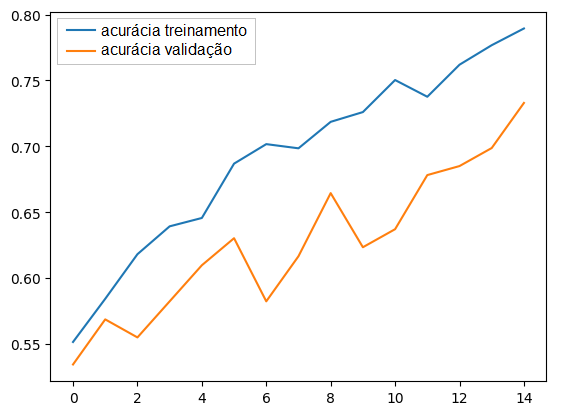
\includegraphics[width=\linewidth]{figuras/accuracy.png}
  \captionsetup{justification=centering}
  \vspace{-0.2cm}
  \\\textbf{\footnotesize Fonte: Elaborado pelos autores}
  \label{fig:acc}
\end{minipage}\hfill
\begin{minipage}{0.45\textwidth}
  \centering
  \caption[\hspace{0.1cm}Grade Computacional.]{Gráfico de perda}
  \vspace{-0.4cm}
  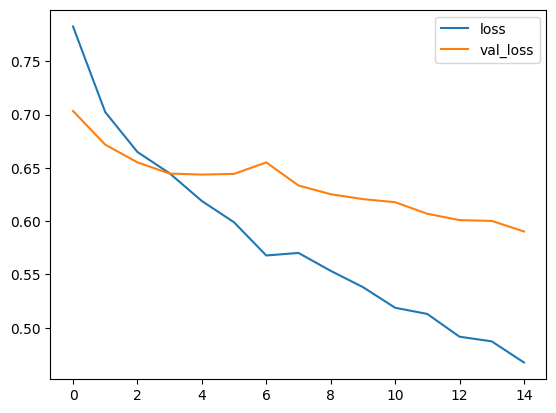
\includegraphics[width=\linewidth]{figuras/loss.png}
  \captionsetup{justification=centering}
  \vspace{-0.2cm}
  \\\textbf{\footnotesize Fonte: Elaborado pelos autores}
  \label{fig:loss}
\end{minipage}
\end{figure}



Em adição, foi gerada uma Matriz de Confusão, disponível para visualização na Tabela \ref{tab:confusion}. Essa matriz revela que o modelo alcançou 104 verdadeiros positivos, indicando sua capacidade de identificar corretamente casos de câncer. Da mesma forma, os 135 verdadeiros negativos evidenciam sua habilidade em reconhecer corretamente situações sem a presença da condição. No entanto, a presença de 130 falsos positivos e 95 falsos negativos destaca desafios na precisão do modelo, representando erros do Tipo I e Tipo II, respectivamente.

\begin{table}[h]
  \centering
  \caption{Matriz de confusão}
   \label{tab:confusion}
   \vspace{-0.2cm}
\begin{tabular}{|c|c|c|c|c|} 
  \hline
     & \textbf{Com câncer} & \textbf{Sem câncer}  \\
  \hline
    \textbf{Com câncer} & 104 & 130 \\
  \hline
    \textbf{Sem câncer} & 95 & 135 \\
  \hline
\end{tabular}
	\vspace{0.2cm}
     \\\textbf{\footnotesize Fonte: Elaborado pelos autores}
\end{table}


% No cenário atual, métricas derivadas da matriz de confusão, como precisão, sensibilidade e pontuação F1, oferecem uma visão mais abrangente do desempenho do modelo. A precisão, calculada como 104 / (104 + 130), oferece uma medida da exatidão das classificações positivas. A sensibilidade, calculada como 104 / (104 + 95), revela a proporção de casos positivos identificados corretamente. 

% \begin{table}[h]
%   \centering
%   \caption{Métricas}
%    \label{tab:metricas}
%    \vspace{-0.2cm}
% \begin{tabular}{|c|c|c|c|c|} 
%   \hline
%     Classificação & Precisão & Sensibilidade & Pontuação F1 & Acurácia \\
%   \hline
%     Com câncer & 0.52 & 0.44 & 0.48 &\\
%   \hline
%     Sem câncer & 0.52 & 0.44 & 0.48 &\\
%   \hline
% \end{tabular}
% 	\vspace{0.2cm}
%      \\\textbf{\footnotesize Fonte: Elaborado pelos autores}
% \end{table}


% No atual cenário, métricas derivadas da matriz de confusão, como sensibilidade, especificidade e precisão, oferecem uma visão mais abrangente do desempenho do modelo. A sensibilidade, calculada como 104 / (104 + 95), revela a proporção de casos positivos identificados corretamente. A especificidade, determinada por 135 / (135 + 130), reflete a capacidade do modelo em reconhecer corretamente casos negativos. Já a precisão, calculada como 104 / (104 + 130), oferece uma medida da exatidão das classificações positivas. Essas métricas contribuem para uma compreensão aprofundada do modelo, essencial para aprimorar sua eficácia na detecção precoce de câncer.





% A interpretação desses números depende do contexto específico do problema. No entanto, algumas métricas comuns derivadas da matriz de confusão incluem:

% Sensibilidade (ou Recall): Proporção de casos positivos que foram corretamente identificados pelo modelo. Calcula-se como TP / (TP + FN). Neste caso, seria 104 / (104 + 95).

% Especificidade: Proporção de casos negativos que foram corretamente identificados pelo modelo. Calcula-se como TN / (TN + FP). Neste caso, seria 135 / (135 + 130).

% Precisão: Proporção de casos identificados como positivos que são realmente positivos. Calcula-se como TP / (TP + FP). Neste caso, seria 104 / (104 + 130).

% Essas métricas ajudarão a fornecer uma compreensão mais detalhada do desempenho do seu modelo em relação à detecção de câncer






%%%%%%%%%%%%%%%%%%%%%%%     PREDIÇÕES       %%%%%%%%%%%%%%%%%%%%%%

\subsection{\esp Predições} \label{pred}

Por fim, procedeu-se à avaliação do modelo de classificação utilizando dados do conjunto de imagens de teste. O resultado da predição para um paciente sem câncer, conforme ilustrado na Figura \ref{fig:predicao_sem}, demonstra uma classificação precisa, identificando corretamente a imagem como pertencente a um paciente sem câncer. No entanto, na Figura \ref{fig:predicao_com}, observou-se uma classificação incorreta, onde o modelo erroneamente indicou que um paciente sem câncer estava com a doença. Esta discrepância é atribuída à limitada acurácia do modelo na classificação de imagens.

\begin{figure}[ht]
\centering
    \begin{minipage}[b]{0.45\textwidth}
        \centering
        \caption{Predição de paciente sem câncer}
        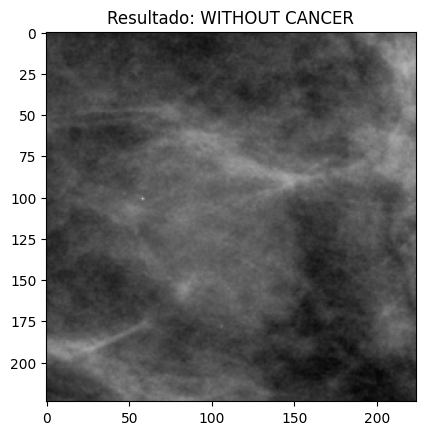
\includegraphics[width=\textwidth]{figuras/predicao_sem.png}
        \label{fig:predicao_sem}
         \textbf{\footnotesize Fonte: \href{https://www.kaggle.com/datasets/awsaf49/cbis-ddsm-breast-cancer-image-dataset}{\cite{newdatabase}}}
    \end{minipage}
    \hfill
    \begin{minipage}[b]{0.45\textwidth}
        \centering
        \caption{Predição de paciente com câncer}
        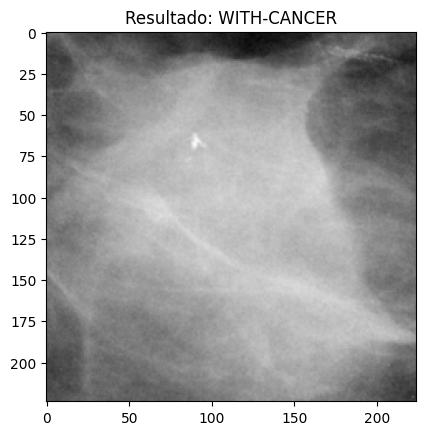
\includegraphics[width=\textwidth]{figuras/predicao_com.png}
        \label{fig:predicao_com}
        \textbf{\footnotesize Fonte: \href{https://www.kaggle.com/datasets/awsaf49/cbis-ddsm-breast-cancer-image-dataset}{\cite{newdatabase}}}
    \end{minipage}
\end{figure}


%%%%%%%%%%%%%%%%%%%%%%%%%%%%%%%%%%%%%%%%%%%%%%%%%%%%%%%%%%%%%%%%%%%%%%%%%
%%%%%%%%%%%%%%%%%%%%%%%%%      CONCLUSÃO      %%%%%%%%%%%%%%%%%%%%%%%%%%%
%%%%%%%%%%%%%%%%%%%%%%%%%%%%%%%%%%%%%%%%%%%%%%%%%%%%%%%%%%%%%%%%%%%%%%%%%


\section{\esp Conclusão} \label{conclusion}
Baseando-se na existência de ferramentas auxiliares no diagnóstico do câncer de mama, o presente artigo propõe uma abordagem que utiliza \textit{Transfer Learning} em redes neurais para a identificação de câncer de mama em pacientes. A proposta visa integrar algoritmos de processamento de imagem, juntamente com estruturas de neurônios como Redes Convolucionais e Redes Residuais, na criação de um modelo de predição. 

Para obter um modelo de predição satisfatório, o procedimento metodológico incluiu o pré-processamento das imagens, envolvendo redimensionamento e definição de \textit{batches} para otimizar a entrada no modelo. Adotou-se a técnica de \textit{Transfer Learning}, incorporando uma Rede Neural Residual (\textit{ResNet-50}) para aprimorar a eficiência no treinamento e resolver problemas associados à degradação de desempenho. Juntamente, foram adicionadas novas \textit{layers}, uma vez que a \textit{ResNet50} não implementa camadas \textit{Fully Connected}, responsáveis por transformar características extraídas em uma saída final. Com a inclusão de novas camadas, o treinamento do modelo foi possibilitado, utilizando funções de otimização e perda.

% colocar mais resultados aqui
Os resultados obtidos durante a validação revelam uma taxa de acurácia de 73\%, indicando a capacidade do do modelo em reconhecer padrões representativos de malignidade em imagens mamográficas. 


Embora resultados tenham sido alcançados, a evolução contínua do estudo em trabalhos futuros visa aprimorar a robustez e aplicabilidade do modelo de detecção de câncer de mama. A incorporação da Validação Cruzada (do inglês \textit{Cross-Validation}) é essencial para avaliar a estabilidade e generalização do modelo. Ao dividir o conjunto de dados em subconjuntos, a técnica permite treinar e validar o modelo várias vezes em diferentes combinações de conjuntos de treinamento e validação, garantindo uma avaliação mais robusta do desempenho, minimizando a possibilidade de \textit{Overfitting}.

Outrossim, o modelo atual retorna uma classificação binária indicando a presença ou ausência de câncer de mama. Em futuras iterações, planeja-se expandir essa abordagem introduzindo uma categorização mais refinada, identificando o estágio ou grau do câncer detectado, permitindo uma análise mais detalhada da condição do paciente.

Ademais, a remoção de ruídos e a segmentação de imagens são processos essenciais para o futuro. Esses processos aprimoram a eficácia da análise ao concentrar-se em regiões de interesse específicas. A remoção de ruídos, realizada por meio de métodos avançados como filtros de suavização, contribui para a obtenção de dados mais limpos e confiáveis. Simultaneamente, a segmentação possibilita uma compreensão mais detalhada da estrutura da imagem, tornando-a mais acessível aos modelos de predição. Assim, a integração desses processos visa otimizar a qualidade dos dados e elevar o desempenho geral do modelo.